
\chapter{Materiais e Métodos}
\label{metodologia}
Este capítulo descreve as tecnologias e etapas para o desenvolvimento
do sistema proposto neste trabalho.

\section{Tecnologias utilizadas}
\label{tecnologias-usadas}

\subsection{Comunicação Wi-Fi e \emph{probe request}}
\label{wifi}

Segundo \citeonline{Teleco2008}, uma Wireless LAN (WLAN) é uma rede local sem
fio padronizada pelo IEEE 802.11. É conhecida também pelo nome de Wi-Fi,
abreviatura de \emph{wireless fidelity} (fidelidade sem fios) e marca registrada
pertencente à Wireless Ethernet Compatibility Alliance (WECA).

De acordo com \citeonline{SIMOES2015}, a tecnologia Wi-Fi é muito utilizada em
sistemas de posicionamento indoor, pois não existe a necessidade de criar uma
infraestrutura de comunicação: em praticamente todos os espaços fechados com
afluência de pessoas, existe já uma criada. Vale ressaltar, porém, que redes
Wi-Fi estão sujeitas a pontos cegos (desvios de sinal em áreas não atingidas
pela rede) - isso pode ser causados por interferências de outros equipamentos,
objetos, fiação elétrica ou mesmo paredes. Dispositivos a uma mesma distância de
um ponto de acesso podem receber qualidades de sinal diferentes.

Ainda segundo \citeonline{SIMOES2015}, um campo de informação que pode ser
recolhido pelos dispositivos móveis é o MAC Address, que permite identificar, na
rede, o AP ao qual o aparelho está ligado, característica esta utilizada no
desenvolvimento deste trabalho.

Como explanado por \citeonline{Teleco2016}, para permitir que uma estação móvel
comunique-se com outras em uma rede IBSS (Independent Basic Service Set) ou um
AP em uma rede infra-estrutura BSS (Basic Service Set), ela deve primeiramente
encontrá-las - processo conhecido como \emph{varredura}. Esse processo pode ser de 2
tipos: passivo, modalidade envolvendo somente a ``escuta'' de tráfego; e ativo
(método utilizado neste trabalho), no qual a estação X executa uma varredura
para extrair informações das demais estações e dos AP’s, economizando tempo.
Para tanto, a estação ativamente transmite \emph{queries} (perguntas para
extrair as respostas das estações numa BSS), movendo-se então para um canal e
transmitindo um pacote do tipo \emph{probe request} (requisição de sondagem): se
houver BSS no canal que coincida com o SSID (Service Set Identifier) do quadro
``requisição de sondagem'', a estação irá responder, enviando um quadro
\emph{probe response} (resposta de sondagem) para a estação que fez a pergunta.

O \emph{probe request} é utilizado como meio de detecção de pessoas, pois
independe da tecnologia do tipo de estação móvel (dispositivo móvel) e está presente em todo lugar (trivial). Ainda, há muitos projetos que já fazem essa detecção através do Tshark, ou seja: há ampla documentação.

Para conectividade Wi-Fi do dispositivo Raspberry Pi, utilizamos o adaptador Ralink MT7601U, do fabricante MediaTek, seguindo o padrão IEEE 802.11:b/g/n (informações de \citeonline{MediaTek}).

Segundo \citeonline{Morimoto2009}, uma das grandes dúvidas ao se montar uma rede wireless é o seu alcance efetivo, o qual sofre grande variação. O valor prometido pela maioria dos fabricantes é de 30 metros em ambientes fechados e 150 metros em ambientes abertos. Devido ao uso de mais transmissores e antenas, o padrão 802.11n oferece um alcance um pouco maior: promete até 70 metros em ambientes fechados e 250 metros em campo aberto. Porém, estes valores são estimados, gerados em testes padronizados: em situações reais, é possível que, em links de longa distância (30 km), clientes não consigam manter uma transmissão estável num ponto de acesso localizado a apenas 6 a 8 metros de distância.

Três fatores explicam diferenças tão grandes: o ganho das antenas utilizadas no ponto de acesso e do cliente, a potência dos transmissores e, principalmente, fontes de interferência presentes no ambiente.

Para \citeonline{Morimoto2009}, os obstáculos que mais depreciam a qualidade do sinal em uma rede são:

\begin{itemize}
  \item superfícies metálicas, como grades, janelas, portas metálicas, lajes, vigas. O metal reflete a maior parte do sinal;
  \item materiais densos, como concreto e pedra;
  \item corpos com grande concentração de líquido, como aquários, piscinas, caixas d'água;
	\item focos de interferência, que competem com o sinal do ponto de acesso;
	\item fornos de microondas, telefones sem fio, transmissores bluetooth e outros aparelhos que operam na faixa dos 2.4 GHz (mesma das redes wireless);
  \item interferência entre diferentes redes instaladas na mesma área
\end{itemize}

Portanto, a combinação de todos esses fatores faz com que o alcance varie muito de acordo com o ambiente, não sendo possível pré-estabelecer um valor fixo que estipule o alcance da antena.

\subsection{Modo monitor}
\label{modo-monitor}
Para que um dispositivo móvel seja identificado independente de qualquer rede ou AP, é essencial que o sistema de detecção possua uma placa e/ou adaptador de rede (NIC) que possa ser habilitado para o modo monitor.

Geralmente, uma interface de rede qualquer captura pacotes dos tipos \emph{managed} e \emph{beacons} que são originados por APs. Estes pacotes são transmitidos
muitas vezes por segundo por APs para indicar quais redes estão realizando \emph{broadcasting}. O modo monitor (\emph{monitor mode}) é um modo de operação em que um NIC consegue capturar todos os tipos de pacotes sem estar associado a um AP \cite{Acrylic} \cite{Wireshark2017b}. Dessa forma, é possível capturar todos os tipos, como os de \emph{probe request} que são enviados de dispositivos móveis.

Neste trabalho, um Raspberry Pi com um adaptador Wi-Fi habilitado no modo monitor captura pacotes \emph{probe request} de dispositivos móveis
para que ocorra a identificação de indivíduos.

\subsection{Tshark}
\label{tshark-section}
O protocolo Tshark é a versão de terminal do protocolo
analisador de rede Wireshark \cite{Wireshark2017} \cite{Wireshark2017a}. Ele é
utilizado para analisar e filtrar (\emph{sniff}) os
pacotes capturados. Esse protocolo foi
escolhido, pois permite realizar o estudo da rede a partir do recebimento de
pacotes e seus campos, além de possuir ampla documentação, maturidade e exemplos
por ser uma tecnologia aberta. Um exemplo de seu uso é o comando a seguir.

\begin{center}
\emph{tshark -i wlan1 -T fields -e wlan.sa -e frame.time}
\end{center}

Cada parte do comando anterior significa:
\begin{itemize}
  \item \textbf{wlan1}: interface de rede que indica a antena Wi-Fi utilizada;
  \item \textbf{wlan.sa}: mostra o endereço MAC do dispositivo que enviou o pacote (em inglês, \emph{source address});
  \item \textbf{frame.time}: mostra a hora, dia e ano em que o pacote foi capturado;
\end{itemize}

A saída no terminal do comando apresentado está na \autoref{saida-comando}.

\begin{figure}[htb]
  \caption{\label{saida-comando}Saída após execução de comando Tshark}
  \begin{center}
    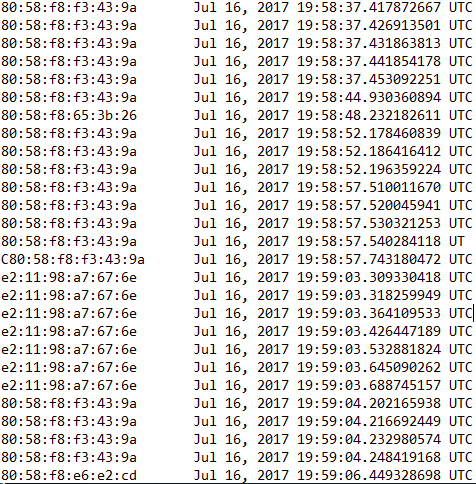
\includegraphics[width=0.90\textwidth]{img/packets.png}
  \end{center}
  \legend{Fonte: Elaborada pelas autoras.}
\end{figure}

\subsection{Raspberry Pi}
O Raspberry Pi é um computador do tamanho de um cartão de crédito que pode ser conectado a monitores, teclados, mouse e outros dispositivos.
Para a detecção de dispositivos móveis um Raspberry Pi Model 3 B juntamente com um adaptador Wi-Fi são utilizados. O Raspberry foi escolhido
pois oferece interface amigável de programação (terminais gráfico e de texto); possui poder de processamento para receber os milhares de pacotes, pré-processá-los
e enviar para o servidor; além de entrada USB para receber uma antena Wi-Fi e também por seu tamanho pequeno \cite{rpi2017}.

Outras opções foram consideradas por serem baratas, acessíveis e terem documentação aberta. Foi o caso do ESP8266 que possui um tamanho extremamente
reduzido e possui o custo médio de R\$15,00 \cite{Embarcados2015}, mas seu uso para este trabalho fica impossibilitado, pois essa tecnologia não consegue ser habilitada para o modo monitor da interface de rede \cite{Puhl2016} \cite{Ferreira2016}.

Uma antena Wi-Fi (Ralink MT7601U) foi equipada no Raspberry para ampliar o alcance da captura já que o propósito do sistema é detecção em zonas que podem
apresentar esparcidade (espalhamento) de indivíduos e ela pôde ser habilitada para o modo monitor (\autoref{modo-monitor}). A antena nativa
do Raspberry não conseguiu ser habilitada para o \emph{monitor mode}.

O sistema operacional utilizado com esta ferramenta foi o Kali Linux, pois,
dentre os sistemas testados, foi o que suportou \emph{drivers} para a antena
Ralink utilizada. Outro ponto é que este SO foi projetado para experimentos e
projetos relacionados à redes de computadores, então possui ampla documentação e exemplos nesse sentido
\cite{kali}.

\subsection{Node.js}
O Node ou Node.js é um \emph{runtime} que permite a execução Javascript fora dos navegadores, nesse caso do lado dos servidores \cite{node}.
Essa ferramenta permite a criação de APIs com entradas e saídas (I/O) não bloqueantes, ou seja, emprega programação assíncrona \cite{Dzone}. Para tal, essa tecnologia é orientada a eventos, assim que um evento ocorre funções específicas são
acionadas para tratá-lo. Nesse cenário, os comandos executam em paralelo utilizando funções de \emph{callback}. Para o sistema proposto nesse trabalho, é uma característica muito importante, já que se trata de um "sistema quase em tempo real", ou seja, é possível atender todas as requisições feitas pelo usuário para a visualização dos dados, como
a postagem de arquivos provenientes do módulo sensor (\autoref{secao-sensor}).

No GSMART, o Node é utilizado tanto na parte do servidor como na parte que executa os comandos do Tshark dentro do Kali Linux, demonstrando ainda mais sua versatilidade.

Outro componente importante do Node é a importação de pacotes produzidos pela comunidade aberta através do gerenciador de pacotes NPM (Node
Package Manager), sendo essencial para facilitar e agilizar a programação. Por exemplo, o servidor deste projeto é baseado no pacote Express.js.

O Express.js é um \emph{framework} que fornece conjunto robusto para aplicativos
web, como: métodos HTTP e \emph{middleware} \cite{express}. Na \autoref{express} é
possível observar um exemplo de tratamento de uma rota de acesso a uma aplicação.
Para importar este pacote, basta abrir o terminal no diretório do projeto e executar o comando
\emh{npm install --save express}.

\begin{figure}[htb]
  \caption{\label{express}Código utilizando Express.js}
  \begin{center}
    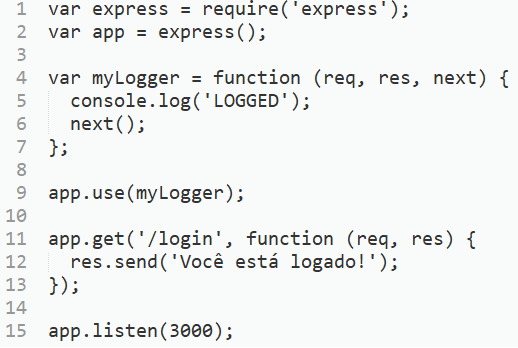
\includegraphics[width=0.70\textwidth]{img/express.png}
  \end{center}
  \legend{Fonte: Elaborada pelas autoras.}
\end{figure}

Na linha 1, importa-se o pacote. Já na linha 11, ele faz o tratamento da rota "login", caso o usuário tente acessá-la (método GET), será retornado uma mensagem de "Você está logado!". Na linha 15, o servidor está escutando a porta 3000 para acesso. Esse trecho de código é um exemplo de como a programação
com Node e seus pacotes por ser simplificada.

O último ponto para a escolha do Node.js foi o fato dele ser baseado na
\emph{engine} V8 de Javascript do Google Chrome, possibilitando utilizar
Javascript tanto para o servidor quanto no lado do cliente.

\subsection{MongoDB}
O MongoDB é um banco de dados NoSQL baseado em coleções de documentos. O número
de campos, conteúdo e tamanho de cada documento pode ser diferente \cite{mongo}.
Cada um desses documentos é representado por um objeto javascript (JSON). Além
disso, o MongoDB oferece API que fornece \emph{queries} rápidas e semelhantes ao
SQL.

Este banco de dados foi utilizado no projeto devido a representação dos dados em
JSON, já que a aplicação é inteiramente em Javascript, ou seja, facilita a
manipulação pelas funções. Outro ponto é a escalabilidade, uma vez que no início
do projeto o custo de uma \emph{query} e o tamanho em \emph{bytes} da unidade do
dado não eram conhecidos. Além disso, optou-se por um banco não-relacional, pois os dados utilizados organizados em tabelas consumiriam demasiado desempenho da aplicação. O modelo de dado será apresentado no \autoref{arq-cap}.

Por fim, os documentos do MongoDB foram manipulados pelo Node.js através do pacote Mongoose que proporciona variadas
funções para abstrair as \emph{queries}.

\section{Métodos e Etapas}
\label{metodos-etapas}

A implementação deste trabalho seguiu 4 etapas. Inicialmente, foi feito o levantamento teórico acerca de \emph{geomarketing} - devido à abrangência do tema, fez-se necessário definir
qual seria o viés a ser seguido. Decidiu-se focar o desenvolvimento em conceitos
relativos à contagem de pessoas e aferição de tráfego local. Foi realizado
também um levantamento bibliográfico a respeito de empresas e projetos
semelhantes ao proposto nesta monografia.

A segunda etapa envolveu a escolha dos materiais e tecnologias a serem
utilizados na concepção de um contator de pessoas. Foram realizados testes de
compatibilidade entre hardware e Sistema Operacional - no caso, utilizando-se
como base o dispositivo portátil Raspberry Pi conforme
\autoref{tecnologias-usadas}. Fizeram-se testes para encontrar o SO adequado às
necessidades do projeto, além de testes para escolha de uma antena Wi-Fi
compatível com as especificações tecnológicas, uma vez que a antena nativa do
Raspberry Pi não funcionou em modo monitor, algo imprescindível na captura de
pacotes de \emph{probe request}. Após selecionar hardware e SO (Kali Linux e antena Ralink), foram escolhidas as demais
tecnologias e ferramentas a serem usadas no desenvolvimento da aplicação e
visualização de dados, que se daria em forma de um \emph{webserver}: linguagens
de programação, bancos de dados e servidores.

Na terceira etapa, desenvolveu-se o módulo de visualização de dados da aplicação.
Primeiramente, construiu-se um servidor em Node.js e sua hospedagem num servidor em nuvem (Digital Ocean). Posteriormente, decidiu-se quais seriam as informações relevantes para serem extraídas dos dados, e construiu-se o layout: foram utilizados HTML, CSS, Javascript, EJS (Embedded
JavaScript - template para apresentação de dados) e Boostrap em forma de
\emph{dashboard} para apresentar gráficos e resumo das informações. Após isso, o
MongoDB foi definido como banco de dados - utilizando-se de sua forma de
organização (coleções e documentos), definiu-se o formato do dado (objetos e
atributos). Por fim, os modelos de preparação e mineração  de dados e o
tratamento de rotas para acesso aos conteúdos do webserver (rotas de GET) e
postagem de arquivos (rotas de POST) foram desenvolvidos.

A última etapa concentrou-se em desenvolver o sensor de detecção com o
Raspberry Pi e a antena Ralink para adequar-se ao modelo de dado definido na
etapa anterior. Desenvolveu-se um \emph{script} que configura a antena para o
modo monitor, inicia a varredura (executando o Tshark) e envia os arquivos
gerados para o servidor. Nesta etapa, o programa foi aperfeiçoado aos poucos,
testando a comunicação entre o Raspberry Pi e o servidor, e se a formatação dos
arquivos enviados e tempo de captura estavam corretos.

De modo geral, a aplicação foi testada durante/a cada etapa - inicialmente,
a partir de dados fictícios, criados no banco de dados. Posteriormente, os testes
prosseguiram com os dados das inúmeras capturas realizadas.

Os principais objetivos nos testes foram:

\begin{itemize}
  \item verificar comunicação entre módulos. Por exemplo: envio de dados do sensor para o servidor, e captura dos pacotes;
  \item tempo de resposta de \emph{requests} para servidor;
  \item garantir programação assíncrona, que é o paradigma do Node.js;
  \item gerar arquivos que fossem corretamente enviados;
  \item garantir que a informações extraídas estivessem corretas do ponto de vista estatístico;
  \item tratar todos os tipos de erros encontrados e supostos problemas para não haver quebra no funcionamento de nenhum módulos (tratamento de exceções);
  \item garantir que o formato de dado manipulado fosse mantido em toda a aplicação, sem necessidade de muitas adaptações nos módulos.
\end{itemize}

Além da fase de desenvolvimento, houve a fase de testes para aferir a precisão de medição do GSMART (veja \autoref{resultados-discussao}).
